\documentclass[a4paper, 11pt]{article}

\usepackage[utf8]{inputenc}
\usepackage{multicol}
\usepackage{graphicx}
\usepackage{float}

\newcommand{\specialcell}[2][c]{\begin{tabular}[#1]{@{}c@{}}#2\end{tabular}}

\title{Working Title}

\author{Chris Morgan}

\date{\today}

\begin{document}
\maketitle

\begin{abstract}
With an increasing percentage of the population living a low intensity and sedentary lifestyle, there is a need to motivate these people to engage in physical exercise. Not only is physical wellbeing affected by a lack of exercise, mental capacity also diminishes faster over time. Exergames are not a new solution to this issue, but most in existence try to emulate the physical activity rather than use it solely as a game mechanic.

We propose to develop an exergame system that is not grounded in reality, while still using a familiar exercise in a relatable context. The game will include an integrated scaling system that balances solo gameplay whilst playing. There will also be multiplayer options to engage with people motivated by competition with others rather than oneself.

To evaluate the exergame we developed, user testing was carried out and compared with other means of physical exercise. This was done through both exergames and real world activity. The exergame proved to be effective at providing them with an enjoyable videogame that incorporates physical activity. It also increased their desire to exercise outside of the study. Additional observations show that exergames less attached to reality, while still being recognisable as exercise, were more enjoyable and motivating than games with closer ties to reality.
\end{abstract}

\clearpage

\section{Introduction}
\begin{multicols}{2}

Regular exercise of moderate intensity is a proven means to reduce incidence of obesity as well as provide benefits for mental capacity and fluidity. Even with these benefits, only half the population are partaking in regular exercise \cite{ministry2013new}. This could be one of the reasons for just under a third of the population being obese and a further third overweight \cite{ministry2013new}.

With obesity and related ailments alone estimated cost \$8 billion over the next decade \cite{lal2012health}, a lack of exercise is not only causing problems with our health but is putting major strain on the economy. A consequence of exercise not being motivating \cite{bartholomew2005college} is that individuals are not exercising enough or at a level of sufficient intensity.

Exergaming is a genre of videogames that integrate exercise into the core gameplay. The genre is an attempt to distract users from the exercise as a means to increase motivation. Research has been done into what motivates people to exercise, whether goal based games are effective \cite{jin2010does}, performance differences in exergaming vs pure exercise \cite{kraft2011heart,maddison2009feasibility}, among other areas. Current research is lacking a solution to problem with motivation. In particular, studies are lacking in the area of competitive multiplayer.

In this paper we will be filling in these gaps in the research, focusing on competitive, multiplayer exergames and the behaviour of individuals whilst playing them.

A few questions arise from the idea of multiplayer exergames:

\begin{enumerate}
	\item Does competitive multiplayer increase motivation and/or performance in exergames?
	\item Are people more motivated by/perform better with live competition or a highscore orientated goal.
\end{enumerate}

Evaluating how individuals react to competition in exergames would provide insight into how to develop exergames that are more engaging for users. 

Testing the difference in performance and motivation of players between two competitive systems is a complicated problem in itself to solve. The two systems will involve competing against another player or competing against the `ghost' of the current high score. In reality, in both systems the test subject will be competing against the `ghost' of a previous run by someone else. This placebo is to remove as many variables from the experiment as possible, boiling it down to how people respond to different competitive situations.

\end{multicols}

\clearpage

\section{Related Work}
\begin{multicols}{2}

In 2008 there had not been much research into exergames, specifically the efficacy of using physically interactive videogames as a primary means of exercise had not been quantified. K. Sell, T. Lillie, and J. Taylor \cite{sell2008energy} explored this area, giving insights into how much energy was expended when playing specific exergames. Their research showed that experienced users work at a higher intensity and expend more energy because of this. While this provides evidence that exergames are a viable alternative to pure physical exercise, at least in terms over energy expenditure, it lacks observations on what make an good exergame or how to motivate users.

More recently, this research has been further developed, branching into determining how to improve the energy expenditure of exergames. In a recent proceeding this year, F. X. Chen, A. C. King, and E. B. Hekler \cite{chen2014healthifying} showed that using an exergaming system with the intent of exercise increased player performance and energy expenditure. When primed for gameplay, players performance decreased along with their energy expenditure.

Using the appropriate controller when designing exergames is vitally important, the comfort and mental effort of individuals when using the system determines their enjoyment and motivation to continue using it. T. Park, U. Lee, S. MacKenzie, M. Moon, I. Hwang, and J. Song \cite{park2014human} show that using a stationary cycle provides adequate comfort as a speed controller for exergames. Given the proven efficacy, we use a similar system in our game.

In more closely related works, extensive research has been done into what makes exergames motivating. H. Song, J. Kim, K. E. Tenzek, and K. M. Lee \cite{song2010effects} found that individuals with a competitive nature had increased intrinsic motivation when playing a competitive exergame as apposed to subjects with low competitiveness. In fact, in a competitive setting the subjects with low competitiveness had a detrimental affect on the exercise experience. While this seems obvious it shows that traditional intrinsic motivations translate to exergaming. This can be used to improve user retainment when designing new exergames.

While the current research has explored competitive motivations in exergaming, there has not been any study done into the motivation of live competition vs. a highscore ghost.

\end{multicols}

\clearpage

\section{Design}
\begin{multicols}{2}

To determine if players enjoy exergames where exercise is not the focus of the game, it is necessary to find a game mechanic that is easy to associate with some form of exercise without the exercise being the sole focus of the mechanic. In Working Title, for example, the mechanic of cycling is used to provide rotational motion to a helicopters blades. While cycling is translatable to powering a helicopter, it is so devoid of reality that the focus of the game is piloting the helicopter and the cycling is simply a means to fly.

By adding cognitive tasks to the course, it is possible to determine increases in motivation in players. Initially, they navigate the course without the cognitive exercises and they are added in after a few run throughs.

\subsection{Contributions}

Working Title is a game that involves navigating a helicopter though a pre-designed course. Throughout the course, there are cognitive exercises to force the user to think logically whilst exercising. While the main goal of the game is to complete the course, there are penalties for failing to complete the tasks along the way.

Cognitive tasks included in the course can be as complicated or as simple as required for the audience. To increase players motivation the tasks need to provide mental stimulus without becoming tiresome.

Some examples for such activities are as follows:
\begin{itemize}
	\item Fly through a specifically coloured ring.
	\item Solve basic arithmetic questions.
	\item Complete an arbitrary pattern sequence.
	\item Shoot specific targets from a set.
\end{itemize}

\end{multicols}

\section{Implementation}
\begin{multicols}{2}

Working Title was implemented using the Unity3D game engine. Creating a game from scratch is a huge undertaking especially when complex external elements are involved, such as interacting with an exercycle, an Occulus Rift and joystick. Unity3D provides a strong game engine and a scripting system to allow for rapid development of prototypes. It also has modules to interact with the Occulus Rift, making that integration much simpler.

\end{multicols}
\begin{figure}[H]
\centering
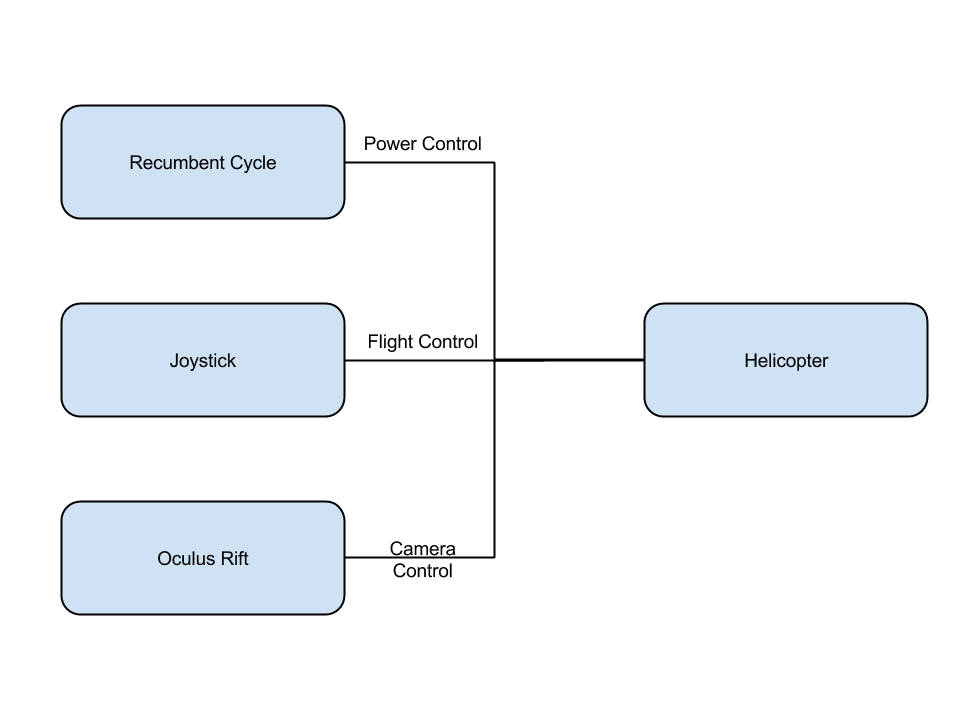
\includegraphics[scale=0.3]{diagram-1.png}
\caption{Control scheme for Working Title}
\end{figure}
\begin{multicols}{2}

To control the helicopter, the player utilities a joystick. This mimics the real world design of how helicopters are controlled. Normally, piloting a helicopter is a complicated activity but the implementation includes stabilisation to help players handle flying. 

The exercise component of the game comes in the form of using a recumbent cycle to control the amount of power applied to the helicopter rotors. This is not only an effective source of physical exertion for the player, but also an idea means to finely control speed and altitude of the helicopter.

An immersive experience is provided having the Occulus Rift as the view window into the game. Players can look around the helicopter cockpit as if they were actually inside it. The Occulus Rift also helps the player have a sense of spatial awareness and helps them judge distances more effectively.



\end{multicols}

\clearpage

\section{Evaluation Methodology}

\subsection{Pre-Questionnaire}

\begin{tabular}{|p{4cm}|c c c c c|}
\hline
Age: &12-17 &18-24 &25-34 &35-44 &45+\\
\hline
Gender: & male & & female & & other \\
\hline
Occupation: & & & & & \\
\hline
\hline
& Daily & \specialcell{Two-Three\\Times a week} & Weekly & Monthly & Never \\
\hline
Have you used an Oculus Rift/VR headset before? & 1 & 2 & 3 & 4 & 5 \\
\hline
Have you used an exercycle/bicycle before? & 1 & 2 & 3 & 4 & 5 \\
\hline
How often do you exercise? & 1 & 2 & 3 & 4 & 5 \\
\hline
How often do you play video games? & 1 & 2 & 3 & 4 & 5 \\
\hline
\hline
& \specialcell{Strongly\\Disagree} & Disagree & Neutral & Agree & \specialcell{Strongly\\Agree} \\
\hline
I consider myself physically fit & 1 & 2 & 3 & 4 & 5 \\
\hline
I feel physically fit today. & 1 & 2 & 3 & 4 & 5 \\
\hline
I enjoy exercising. & 1 & 2 & 3 & 4 & 5 \\
\hline
I enjoy playing video games. & 1 & 2 & 3 & 4 & 5 \\
\hline
\end{tabular}

\vspace{5mm}

\subsection{Post-Case Questionnaire}

\begin{tabular}{|p{4cm}|c c c c c|}
\hline
& \specialcell{Strongly\\Disagree} & Disagree & Neutral & Agree & \specialcell{Strongly\\Agree} \\
\hline
I found the experience physically challenging.& 1 & 2 & 3 & 4 & 5 \\
\hline
I felt comfortable while using the system.& 1 & 2 & 3 & 4 & 5 \\
\hline
I experienced motion sickness while playing the game.& 1 & 2 & 3 & 4 & 5 \\
\hline
I felt challenged physically while using the system.& 1 & 2 & 3 & 4 & 5 \\
\hline
I felt challenged mentally while using the system.& 1 & 2 & 3 & 4 & 5 \\
\hline
Playing the exergame was enjoyable overall.& 1 & 2 & 3 & 4 & 5 \\
\hline
The exergame was immersive.& 1 & 2 & 3 & 4 & 5 \\
\hline
\end{tabular}

\vspace{5mm}

\subsection{Summary Questionnaire}

\begin{tabular}{|p{5cm}|c c c c c|}
 \hline
 & \specialcell{Strongly\\Disagree} & Disagree & Neutral & Agree & \specialcell{Strongly\\Agree} \\
\hline
I enjoyed playing the exergame. & 1 & 2 & 3 & 4 & 5 \\
\hline
I would prefer to exercise using this exergame rather than through traditional means. & 1 & 2 & 3 & 4 & 5 \\
\hline
I found the game with the cognitive exercises more motivating. & 1 & 2 & 3 & 4 & 5 \\
\hline
How do you think the additional task affected your performance? & & & & & \\
& & & & & \\
\hline
Which of the modes of play would you prefer to use as a form of entertainment? & & & & & \\
& & & & & \\
\hline
Which of the modes of play would you prefer to use as a form of exercise? & & & & & \\
& & & & & \\
\hline
Comments and Suggestions? & & & & & \\
& & & & & \\
& & & & & \\
& & & & & \\
& & & & & \\
\hline
\end{tabular}

\clearpage

\bibliographystyle{ieeetr}
\small
\bibliography{References}

\end{document}